It turns out the integral of the gradient of the logarithm can be determined using complex analysis.
The gradient is an operator from the real numbers into the vector space of the complex numbers, in the sense that
\[
\nabla u(\ezh) = \deex u(\ezh) + i\deez u(\ezh), \qquad \ezh = x + iz.
\]
Considering now an analytic function $\uvec = u + iv$, its complex derivative is given by $\partial_{\ezh} \uvec = \deex u + i\deex v$, which by the \textsc{Cauchy}--\textsc{Riemann} equations yields that $\partial_{\ezh} \uvec = {\nabla u}^{\ast}$.
We recall that the principal value of the complex logarithm is given by $\log{(\ezh)} = \ln{\absl{\ezh}} + i\Arg{(\ezh)}$,\footnote{\cite{lavrentev1967methoden} \textsc{Lavrentev} \& \textsc{\v{S}abat}, p.30} so that $\partial_{\ezh} \log{(\ezh)} = {\nabla\ln{\absl{\ezh}}}^{\ast}.$

Now, for a curve parametrized by $\lambda(s)$, the normal vector $\nhat$ may be represented by\footnote{\cite{markusevic1965theoryII} \textsc{Marku\v{s}evi\v{c}}, p.175}
\begin{equation}\label{eq:normal_curve}
\nu(s) = -i \lambda^{\prime}(s) = \frac{\dee z}{\dee s} - i\frac{\dee x}{\dee s} = -i\frac{\dee \ezh}{\dee s}.
\end{equation}
The inner product may be defined such that $\uvec\cdot\nhat = \Re{(\uvec^{\ast} \nu(s))}$.
We then have that
\[
\partial_{\nhat}\ln{r} = \Re{\left( -i\frac{\dee \ezh}{\dee s} \partial_{\ezh} \log{(\ezh - \bzhe_m)} \right)}.
\]
Since the line segment is parameterized by $s$, the differential element may then be taken over $\ezh$.
By the linearity of the $\Re{(\star)}$ operator, we have that
\begin{align*}
  \int_{S_n} \partial_{\nhat} \ln{r} \,\dee S & = -\Re i \int_{{\xvec}_{n-1}}^{\xvec_n} \frac{\dee}{\dee\ezh} \log{(\ezh - \bzhe_m)} \,\dee\ezh.\\
  & = \Arg{\left( \frac{\xvec_{n - 1} - \bzhe_m}{\xvec_n - \bzhe_m} \right)}.
\end{align*}
This is just the angle between $\xvec_n$, $\bzhe_m$, and $\xvec_{n-1}$.
\begin{Figure}
  \centering
  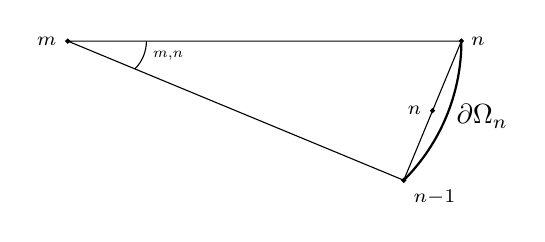
\begin{tikzpicture}
    \begin{scope}[scale = 2.5]
        \def\r{1}\def\smallr{.2}
        \def\thetai{-45}\def\thetaf{0}\def\thetam{180}
        \draw
            (
                {(1-\smallr)*\r*cos(\thetam) + \smallr*\r*cos(\thetaf)},
                {(1-\smallr)*\r*sin(\thetam) + \smallr*\r*sin(\thetaf)}
            ) arc (\thetaf:\thetai:\smallr) node[midway, right]{\scalebox{.75}{$\Thetatt_{m,n}$}};
        \draw[cap = round]
            ({\r*cos(\thetaf)}, {\r*sin(\thetaf)})--
            ({\r*cos(\thetam)}, {\r*sin(\thetam)})--
            ({\r*cos(\thetai)}, {\r*sin(\thetai)})--cycle;
        \draw[thick] ({\r*cos(\thetai)}, {\r*sin(\thetai)}) arc (\thetai:\thetaf:\r) node[midway, right]{${\partial\Omega}_{n}$};
        \draw[fill = black] ({\r*cos(\thetaf)}, {\r*sin(\thetaf)}) circle (.01) node[right]{$\xvec_n$};
        \draw[fill = black] ({\r*cos(\thetai)}, {\r*sin(\thetai)}) circle (.01) node[below right]{$\xvec_{n-1}$};
        \draw[fill = black] ({\r*cos(\thetam)}, {\r*sin(\thetam)}) circle (.01) node[left]{$\bzhe_m$};
        \draw[fill = black]
            (
                {.5*\r*cos(\thetaf) + .5*\r*cos(\thetai)},
                {.5*\r*sin(\thetaf) + .5*\r*sin(\thetai)}
            ) circle (.01) node[left]{$\bzhe_n$};
    \end{scope}
\end{tikzpicture}

  \captionsetup{type = figure}
  \caption{Visualization of $\Thetatt_{m,n}$. Here ${\partial\Omega}_{n}$ denotes the segment along $\partial\Omega$ between $\xvec_{n}$ and $\xvec_{n-1}$.}
\end{Figure}

If $\xtt$ then is the array of the $N$ nodes $x_n$, we can fill the matrix $\Thetatt$ with the arguments with \texttt{for}-loops, which is implemented in the \texttt{assemble} method in the \texttt{IntegralEquation} class, found in \texttt{integralequation.py}.
The class variable $\zhett = \sfrac{1}{2}(\xvec_{n} + \xvec_{n-1})$, containing the aforementioned midpoints is created upon initialization of the class, since multiple methods make use of it.
\begin{algorithm}[H]
    \caption{Assemble $\Thetatt$}\label{alg:theta}
    \begin{algorithmic}
        \For{$\mathtt{m},\mathtt{n} \leq \mathtt{N}$}
            \If{$\mathtt{m} = \mathtt{n}$}
                \State $\Thetatt_{\mathtt{m}\mathtt{n}} \gets -\pi$
            \Else
                \State $\Thetatt_{\mathtt{m}\mathtt{n}} \gets \mathtt{angle}{\left( \frac{\xtt[\mathtt{n}-1] - \zhett[\mathtt{m}]}{\xtt[\mathtt{n}] - \zhett[\mathtt{m}]} \right)}$
            \EndIf
        \EndFor
    \end{algorithmic}
\end{algorithm}
\noindent This method essentially assembles the entire left-hand side of the integral equation, so that we may simply solve $\phi = \Thetatt^{-1}\mathtt{h}$.
